\section{Dynamical Modelling}


%=============================================

\begin{deluxetable*}{lllrl}[!htbp]
\tabletypesize{\scriptsize}
\tablecaption{Gravitational potentials of the reference galaxies used troughout this work and the respective ways to calculate actions in these potentials. All four potentials are axisymmetric. The potential parameters are fixed for the mock data creation at the values given in this table. In the subsequent analyses we aim to recover these potential parameters again. The parameters of \texttt{MW13-Pot} and \texttt{KKS-Pot} were chosen to resemble the \texttt{MW14-Pot} (see Figure \ref{fig:ref_pots}). We use $v_\text{circ}(R_\odot)$ = $230$ km s$^{-1}$ for all potentials in this work. \label{tbl:referencepotentials}}
\tablewidth{0pt}
\tablehead{
\colhead{name} & \colhead{potential type} & \multicolumn{2}{c}{potential parameters $p_\Phi$} & \colhead{action calculation}}
\startdata
\texttt{Iso-Pot}      & isochrone potential\tablenotemark{(a)} & $b$& $0.9~\text{kpc}$ & \textbf{\emph{analytical and exact}} \\
                               & \citep{1959AnAp...22..126H} &                                            &                               & (\citealt{2008gady.book.....B}, \S 3.5.2) \\
\tableline
\texttt{KKS-Pot}    & 2-component                            & $\Delta$                                              & $0.3$   & \textbf{\emph{exact}} \\
                               & Kuzmin-Kutuzov-                      & $\left(\frac{a}{c}\right)_\text{Disk}$ & $20$    & using \emph{St\"{a}ckel Fudge} \\ 
                               & St\"{a}ckel potential\tablenotemark{(b)} & $\left(\frac{a}{c}\right)_\text{Halo}$ & $1.07$ & \citep{2012MNRAS.426.1324B} \\
                               & \hspace{0.3cm} (disk + halo) & $k$                                                       & $0.28$ & and interpolation \\
                               & \citep{1994AA...287...43B}                               &                                                              &               & on action grid \\
                               &                                                       &                                                              &                & \citep{2015ApJS..216...29B,2012MNRAS.426.1324B} \\
\tableline
\texttt{MW13-Pot} & MW-like potential\tablenotemark{(c)} with & $R_d$ & $3~\text{kpc}$ & \textbf{\emph{approximate}} \\ 
                               & Hernquist bulge,                         & $z_h$ & $0.4~\text{kpc}$  & (same as \texttt{KKS-Pot}) \\
                               & spherical power-law halo,        & $f_h$ & $0.5$ & \\
                               & 2 exponential disks                    & $\frac{\diff \ln(v_\text{circ}(R_\odot))}{ \diff \ln(R)}$ & $0$  & \\
                               & \hspace{0.3cm} (stars + gas)  &  & & \\
                               & \citep{2013ApJ...779..115B} & & &\\
\tableline
\texttt{MW14-Pot} & MW-like potential\tablenotemark{(d)} with &  & & \textbf{\emph{approximate}} \\
                               & cut-off power-law bulge, & & & (same as \texttt{KKS-Pot}) \\
                               & Miyamoto-Nagai stellar disk, & & & \\
                               & NFW halo & & & \\
                               & \citep{2015ApJS..216...29B} & & & 
\enddata
\tablenotetext{(a)}{The isochrone potential \texttt{Iso-Pot} has one free parameter, the scale length $b$.} 
\tablenotetext{(b)}{The coordinate system of each of the two St\"{a}ckel-potential components of the \texttt{KKS-Pot} is $\frac{R^2}{\tau_{i,p}+\alpha_p} + \frac{z^2}{\tau_{i,p}+\gamma_p}=1$ with $p \in \{\text{Disk},\text{/Halo}\}$ and $\tau_{i,p} \in \{\lambda_p,\nu_p\}$. Both components have the same focal distance $\Delta \equiv \sqrt{\gamma_p-\alpha_p}$, to make sure that the superposition of the two components itself is still a St\"{a}ckel potential. The axis ratio of the coordinate surfaces $\left(\frac{a}{c}\right)_p := \sqrt{\frac{\alpha_p}{\gamma_p}}$ describes the flatness of the corresponding St\"{a}ckel component. The parameter $k$ describes the relative contribution of the disk mass to the total mass.} 
\tablenotetext{(c)}{The free parameters of the \texttt{MW13-Pot} are stellar disk scale length $R_d$ and height $z_d$, as well as the relative halo contribution to $v_\text{circ}^2(R_\odot)$, $f_h$, and the slope of the rotation curve, $\frac{\diff \ln(v_\text{circ}(R_\odot))}{ \diff \ln(R)}$.} 
\tablenotetext{(d)}{The \texttt{MWPotential2014} by \citet{2015ApJS..216...29B} (see their Table 1) has a circular velocity at the Sun of $v_\text{circ}(R_\odot)$ = $220$ km s$^{-1}$. In this work we use however $v_\text{circ}(R_\odot)$ = $230$ km s$^{-1}$ for all potentials.} 
\end{deluxetable*}

%=============================================

%FIGURE: reference potentials

\begin{figure*}[!htbp]
\includegraphics[width=\textwidth]{figs/reference_potentials.eps}
\caption{Density distribution of the four reference galaxy potentials in Table \ref{tbl:referencepotentials}, for illustration purposes. These potentials are used throughout this work for mock data creation and potential recovery.}
\label{fig:ref_pots}
\end{figure*}


%======================================================================================

%=============================================

\begin{deluxetable*}{lccccc}[!htbp]
\tabletypesize{\scriptsize}
\tablecaption{Reference distribution-function parameters for the qDF in Equations (\ref{eq:df_general})-(\ref{eq:sigmazRg}). These DFs describe the phase-space distribution of stellar populations for which mock data is created and analysed throughout this work for testing purposes. The parameters of the \texttt{cooler} \& \texttt{colder}  (\texttt{warmer}) qDFs were chosen to have the same $\sigma_{R,0}/\sigma_{z,0}$ ratio as the \texttt{hot} (\texttt{cool}) qDF. The \texttt{colder} and \texttt{warmer} qDF have a free parameter $X$ that governs how much colder/warmer they are then the reference \texttt{hot} and \texttt{cool} qDFs. Hotter populations have shorter tracer scale lengths \citep{2012ApJ...753..148B} and the velocity dispersion scale lengths were fixed according to \citet{bov12c}. \label{tbl:referenceMAPs}}
\tablewidth{0pt}
\tablehead{
\colhead{name} & \multicolumn{5}{c}{qDF parameters $p_\text{DF}$}\\
                       & \colhead{$h_R$ [kpc]} & \colhead{$\sigma_{R,0}$ [km s$^{-1}$]} & \colhead{$\sigma_{z,0}$ [km s$^{-1}$]} & \colhead{$h_{\sigma,R}$ [kpc]} & \colhead{$h_{\sigma,z}$ [kpc]}}
\startdata
\texttt{hot}    & 2   & 55 & 66 & 8 & 7\\
\texttt{cool}   & 3.5 & 42 & 32 & 8 & 7\\
\tableline
\texttt{cooler}    & $2  +50\%$ & $55-50\%$ & $66-50\%$ & $8$ & $7$ \\
\texttt{colder}    & $2  +X  \%$ & $55-X  \%$  & $66-X  \%$ & $8$ & $7$ \\
\texttt{warmer} & $3.5-X  \%$ & $42+X  \%$ & $32+X  \%$ & $8$ & $7$
\enddata
\end{deluxetable*}

%=============================================

%============================================

In this section we summarize the basic elements of \RM{}, the dynamical modelling machinery presented in this work, which in many respects follows BR13 and makes extensive use of the \texttt{galpy} Python package\footnote{\texttt{galpy} is an open-source code that is being developed on \url{http://github.com/jobovy/galpy}. The latest documentation can be found at \url{http://galpy.readthedocs.org/en/latest/}.} \citep{2015ApJS..216...29B}.

\subsection{Coordinate System} \label{sec:coordinates}

Our modelling takes place in the Galactocentric rest-frame with cylindrical coordinates $\vect{x} \equiv (R,\phi,z)$ and corresponding velocity components $\vect{v} \equiv (v_R,v_\phi,v_z)$. If the stellar phase-space data is given in observed heliocentric coordinates, position $\tilde{\vect{x}} \equiv(\text{RA},\text{Dec},m-M)$ in right ascension RA, declination Dec and distance modulus $(m-M)$ as proxy for the distance from the Sun, and velocity $\tilde{\vect{v}} \equiv (\mu_\text{RA} \cdot \cos \text{Dec},\mu_\text{Dec},v_\text{los})$ as proper motions $\vect{\mu}=(\mu_\text{RA} \cdot \cos \text{Dec},\mu_\text{Dec})$ in both RA and Dec direction and line-of-sight velocity $v_\text{los}$, the data $(\tilde{\vect{x}},\tilde{\vect{v}})$ has to be converted first into the Galactocentric rest-frame coordinates $(\vect{x},\vect{v})$ using the Sun's position and velocity. We assume for the Sun
\begin{eqnarray*}
(R_\odot,\phi_\odot,z_\odot) &=&(8 \text{ kpc}, 0^\circ, 0 \text{ kpc})\\
(v_{R,\odot},v_{T,\odot},v_{z,\odot}) &=& (0,230,0) \text{ km s}^{-1}.
\end{eqnarray*}

\subsection{Actions and Potential Models}  \label{sec:potentials}

Orbits in axisymmetric potentials are best described and fully specified by the three actions $\vect{J} \equiv (J_R, J_z, J_\phi=L_z)$ (\citealt{2008gady.book.....B}, \S 3.5). Their computation from a star's phase-space coordinates, $(\vect{x},\vect{v}) \longrightarrow \vect{J}$, is typically very expensive and depends on the choice of gravitational potential in which the star moves. The spherical isochrone potential \citep{1959AnAp...22..126H} and axisymmetric St\"{a}ckel potential \Wilma{[TO DO: REF]} are the most general Galactic potentials, that allow exact action calculations (\citealt{2008gady.book.....B}, \S 3.5.2 and [TO DO: REF]). In all other potentials actions have to be numerically estimated, e.g., by using the \emph{St\"{a}ckel fudge} by \citet{2012MNRAS.426.1324B} for axisymmetric potentials and action interpolation grids \citep{2015ApJS..216...29B,2012MNRAS.426.1324B} to speed up the calculation. The latter is one of the improvements employed by \RM{}, which was not used by BR13.

For the gravitational potential in our modelling we assume a family of parametrized potential models. We use: The MW-like potential from BR13 (\texttt{MW13-Pot}) with bulge, disk and halo; the spherical isochrone potential (\texttt{Iso-Pot}); and the 2-component Kuzmin-Kutuzov St\"{a}ckel potential (\citealt{1994AA...287...43B}; \texttt{KKS-Pot}), which also displays a disk and halo structure. Table \ref{tbl:referencepotentials} summarizes all reference potentials used in this work together with their free parameters $p_\Phi$. The density distribution of these potentials is illustrated in Figure \ref{fig:ref_pots}.\\




\subsection{Stellar Distribution Functions} \label{sec:qDF}

A simple DF, which we will employ as a specific example throughout this work to describe individual stellar sub-populations, is the action-based quasi-isothermal distribution function (qDF) by \citet{2010MNRAS.401.2318B} and \citet{2011MNRAS.413.1889B}. This is motivated by the findings of \citet{bov12b,bov12c,2012ApJ...753..148B} and \citet{2013MNRAS.434..652T} about the simple phase-space structure of stellar mono-abundance populations (\MAP{}), and following BR13 and their successful application. The qDF by \citet{2011MNRAS.413.1889B} has the form
\begin{eqnarray}
&&\text{qDF}(\vect{J} \mid p_\text{DF}) \nonumber\\
&&= f_{\sigma_R}\left(J_R,L_z \mid p_\text{DF}\right) \times f_{\sigma_z}\left(J_z,L_z \mid p_\text{DF}\right)\label{eq:df_general}\end{eqnarray}
with some free parameters $p_\text{DF}$ and
\begin{eqnarray}
f_{\sigma_R}\left(J_R,L_z \mid p_\text{DF}\right) &=& n \times \frac{\Omega}{\pi\sigma_R^2(R_g) \kappa}\exp\left(-\frac{\kappa J_R}{\sigma_R^2(R_g)} \right) \nonumber\\
&& \times \left[1+\tanh\left(L_z/L_0\right) \right]\\
f_{\sigma_z}\left(J_z,L_z \mid p_\text{DF} \right) &=& \frac{\nu}{2 \pi \sigma_z^2(R_g)} \exp\left( -\frac{\nu J_z}{\sigma_z^2(R_g)} \right).
\end{eqnarray}
Here $R_g \equiv R_g(L_z)$, $\Omega\equiv \Omega(L_z)$,  $\kappa\equiv \kappa(L_z)$ and $\nu\equiv \nu(L_z)$ are respectively the (guiding-center) radius, circular, radial/epicycle and vertical frequency of the circular orbit with angular momentum $L_z$ in a given potential (\citealt{2008gady.book.....B}, \S 3.2.3). The term $\left[1+\tanh\left(L_z/L_0\right) \right]$ suppresses counter-rotation for orbits in the disk with $L \gg L_0$ (with $L_0 = 10 \times R_\odot/8 \times v_\text{circ}(R_\odot)/220$.
\\Again following BR13, we choose the functional forms
\begin{eqnarray}
n(R_g \mid p_\text{DF}) &\propto& \exp\left(-\frac{R_g}{h_R} \right)\\
\sigma_R(R_g \mid p_\text{DF}) &=& \sigma_{R,0} \times \exp\left(- \frac{R_g-R_\odot}{h_{\sigma,R}} \right)\label{eq:sigmaRRg}\\
\sigma_z(R_g \mid p_\text{DF}) &=& \sigma_{z,0} \times \exp\left(- \frac{R_g-R_\odot}{h_{\sigma,z}} \right)\label{eq:sigmazRg},
\end{eqnarray}
which indirectly set the stellar number density and radial and vertical velocity dispersion profiles. The qDF has therefore a set of five free parameters $p_\text{DF}$: the density scale length of the tracers $h_R$, the radial and vertical velocity dispersion at the solar position $R_\odot$, $\sigma_{R,0}$ and $\sigma_{z,0}$, and the scale lengths $h_{\sigma,R}$ and $h_{\sigma,z}$, that describe the radial decrease of the velocity dispersion. \RM{} allows to fit any number of DF parameters simultaneously, while BR13 kept $\{\sigma_{R,0},h_{\sigma,R}\}$ fixed. Throughout this work we make use of a few example stellar populations whose qDF parameters are given in in Table \ref{tbl:referenceMAPs}: Most tests use the \texttt{hot} and \texttt{cool} qDFs, which correspond to kinematically hot and cool populations, respectively.\\

One crucial point in our dynamical modelling technique (Section \ref{sec:likelihood}), as well as in creating mock data (Section\ref{sec:mockdata}), is to calculate the (axisymmetric) spatial tracer density $\rho_\text{DF}(\vect{x} \mid p_{\Phi},p_\text{DF})$ for a given DF and potential. Analogously to BR13, 
\begin{eqnarray}
&&\rho_\text{DF}(R,|z| \mid p_{\Phi},p_\text{DF}) \nonumber\\
&&= \int_{-\infty}^{\infty} \text{qDF}(\vect{J}[R,z,\vect{v} \mid p_{\Phi}] \mid p_\text{DF}) \Diff3\vect{v}  \\%\label{eq:tracerdensity_general}\\
&&\approx \int_{-n_\sigma \sigma_R(R \mid p_\text{DF})}^{n_\sigma \sigma_R(R \mid p_\text{DF})} \int_{-n_\sigma\sigma_z(R \mid p_\text{DF})}^{n_\sigma \sigma_z(R \mid p_\text{DF})} \int_{0}^{1.5 v_\text{circ}(R_\odot)}  \nonumber\\
& & \hspace{1cm} \text{qDF}(J[R,z,\vect{v} \mid p_{\Phi}] \mid p_\text{DF}) \diff v_T \diff v_z \diff v_R, \label{eq:tracerdensity}
\end{eqnarray}
where $\sigma_R(R \mid p_\text{DF})$ and $\sigma_z(R \mid p_\text{DF})$ are given by Equations \ref{eq:sigmaRRg} and \ref{eq:sigmazRg}.\footnote{The integration ranges over the velocity are motivated by Figure \ref{fig:kks2WedgeEx}. The integration range $[0,1.5 v_\text{circ}(R_\odot)]$ over $v_T$ is in general sufficient, only for observation volumes with larger mean stellar $v_T$ this upper limit needs to be increased.} Each integral is evaluated using a $N_v$-th order Gauss-Legendre quadrature. For a given $p_\Phi$ and $p_\text{DF}$ we explicitly calculate the density on $N_x \times N_x$ regular grid points in the $(R,z)$ plane and interpolate in between using bivariate spline interpolation. The grid is chosen to cover the extent of the observations (for $|z|\geq0$, because the model is symmetric in $z$ by construction). The total number of actions to be calculated to set up the density interpolation grid is $N_x^2 \times N_v^3$, which is one of the speed limiting factors. To complement the work by BR13, we will specifically work out in Section \ref{sec:likelihood} and Figure \ref{fig:norm_accuracy} how large $N_x$, $N_v$ and $n_\sigma$ have to be chosen to get the density with a sufficiently high numerical accuracy. 


\subsection{Selection Functions} \label{sec:selectionfunction}

Any survey's selection function (SF) can be understood as defining an effective sample sub-volume in the space of observables, e.g., position on the sky (limited by the pointing of the survey), distance from the Sun (limited by brightness and detector sensitivity), colors and metallicity of the stars (limited by survey mode and targeting). We use simple spatial SFs, which describe the probability to observe a star at $\vect{x}$,
\begin{eqnarray*}
\text{SF}(\vect{x}) \equiv \begin{cases}
\text{completeness}(\vect{x}) &\text{if $\vect{x}$ within observed volume}\\
0 & \text{outside.}
\end{cases}
\end{eqnarray*}

%====================================================================

%FIGURE: distribution of mock data in action and configuration space

\begin{figure}[!htbp]
\centering
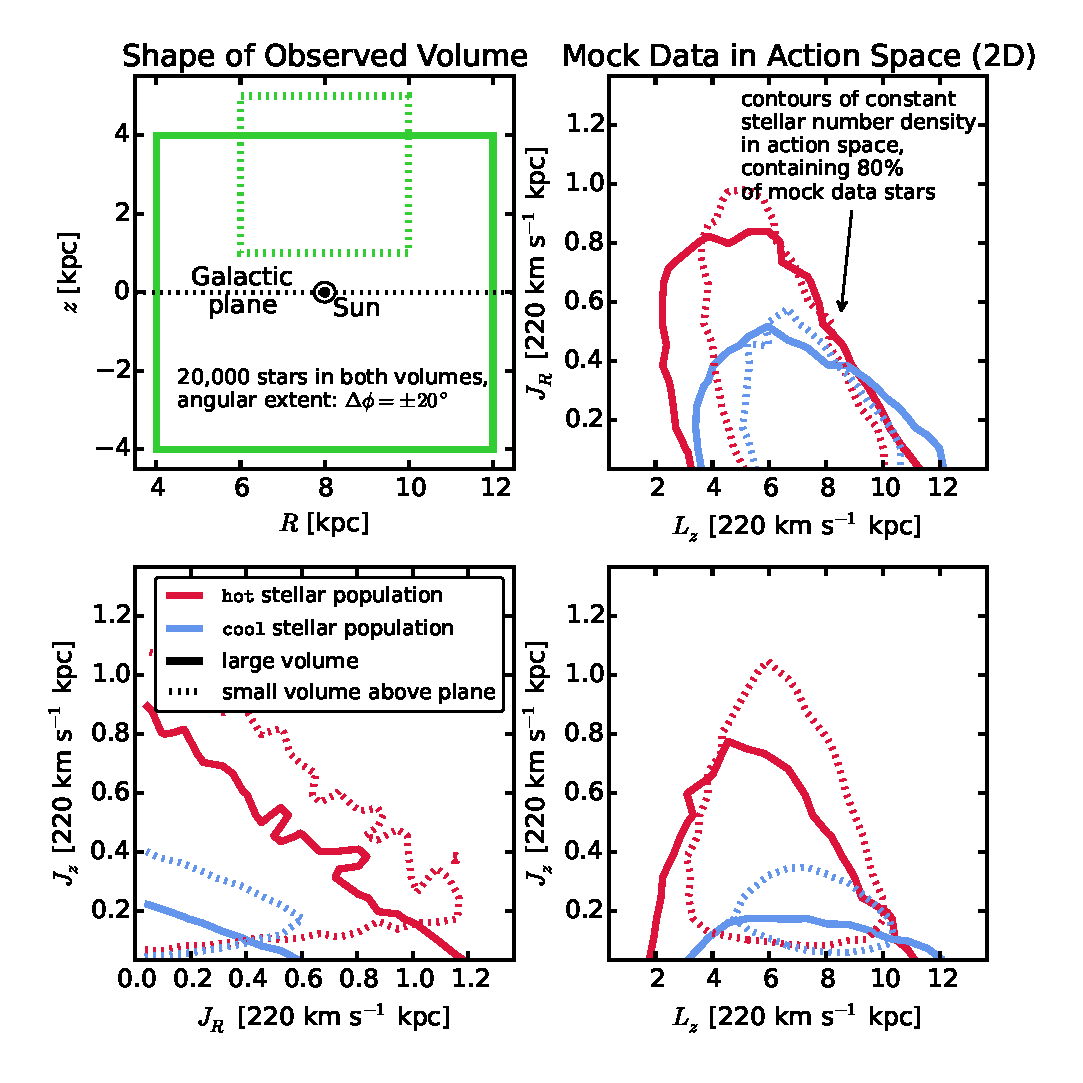
\includegraphics[width=\columnwidth]{figs/kks2WedgeEx_mockdata_actions.eps}
\caption{Distribution of mock data in action space (2D iso-density contours, enclosing 80\% of the stars), depending on shape and position of a wedge-like survey observation volume (upper left panel) and temperature of the stellar population (indicated in the legend). The \pmodel{} of the mock data, created in the \texttt{KKS-Pot} potential, are given as Test \ref{test:kks2WedgeEx} in Table \ref{tbl:tests}. The distribution in action space visualizes how orbits with different actions reach into different regions within the Galaxy. The corresponding mock data in configuration space is shown in Figure \ref{fig:kks2WedgeEx_xv}.} 
\label{fig:kks2WedgeEx_actions}
\end{figure}

\begin{figure}[!htbp]
\centering
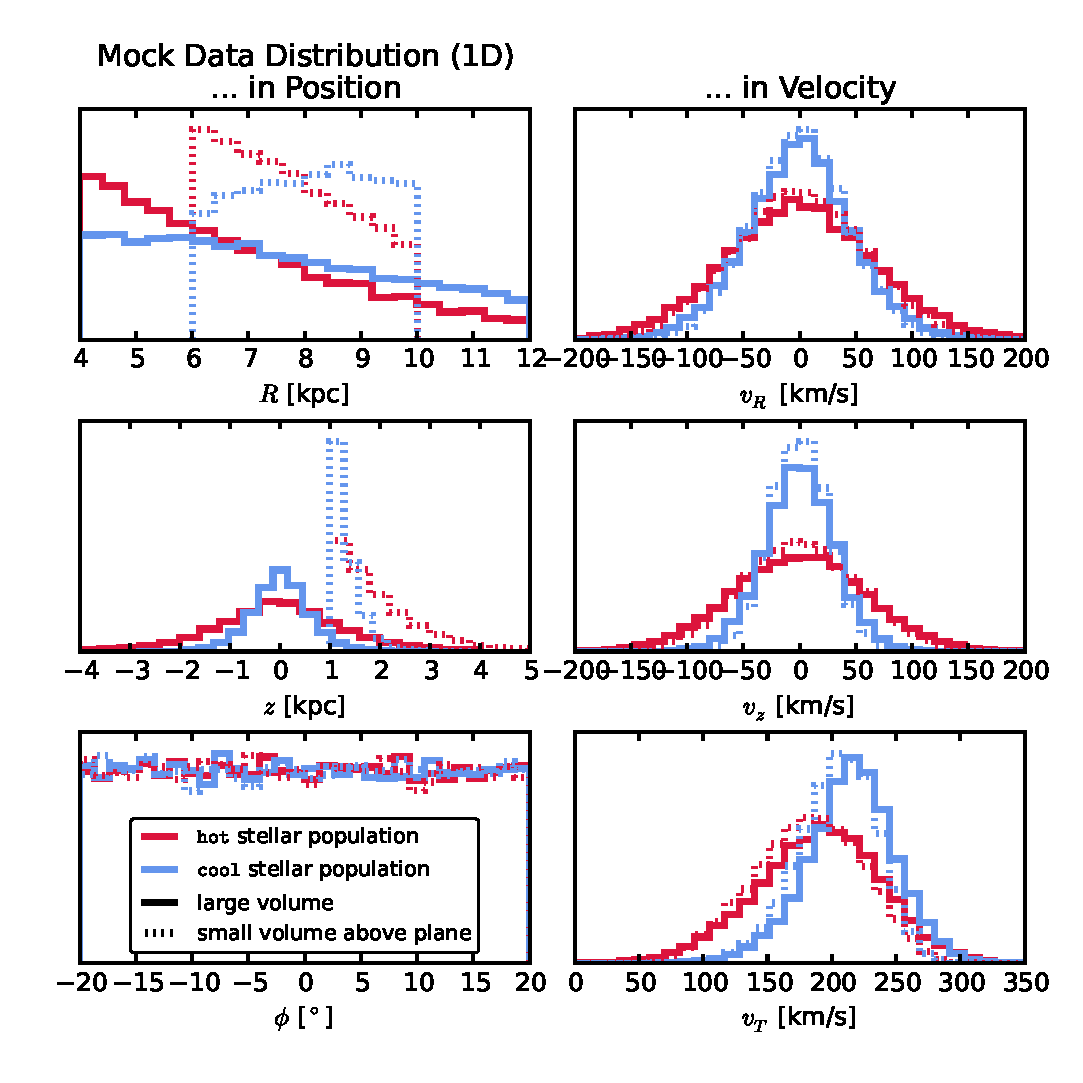
\includegraphics[width=\columnwidth]{figs/kks2WedgeEx_mockdata_xv.eps}
\caption{Distribution of the mock data from Figure \ref{fig:kks2WedgeEx_actions} in configuration space. The corresponding observation volumes (as indicated in the legend) are shown in Figure \ref{fig:kks2WedgeEx_actions}, upper left panel. The 1D histograms on illustrate that qDFs generate realistic stellar distributions in Galactocentric coordinates $(R,z,\phi,v_R,v_z,vT)$: More stars are found at smaller $R$ and $|z|$, and are distributed uniformly in $\phi$ according to our assumption of axisymmetry. The distribution in radial and vertical velocities, $v_R$ and $v_z$, is approximately Gaussian with the (total projected) velocity dispersion being of the order of $\sim\sigma_{R,0}$ and $\sim\sigma_{z,0}$ (see Table \ref{tbl:referenceMAPs}). The distribution of tangential velocities $v_T$ is skewed because of asymmetric drift . \Wilma{[TO DO: Make plot smaller.]}} 
\label{fig:kks2WedgeEx_xv}
\end{figure}

\Wilma{[TO DO: Make sure that mock data plots are referenced everywhere correctly]}

%===========================================================================================================================================================================================



The SF of the SEGUE survey \citep{2012ApJ...753..148B} used by BR13 consists of many pencil-beams. In anticipation of large contiguous volume surveys like Gaia, we use SFs that span large observed volumes of simple geometrical shapes: a sphere of radius $r_\text{max}$ with the Sun at its center; or an angular segment of an cylindrical annulus (wedge), i.e. the volume with $R \in [R_\text{min},R_\text{max}],\phi \in [\phi_\text{min},\phi_\text{max}],z \in [z_\text{min},z_\text{max}]$ within the model Galaxy. The sharp outer edge of the survey volume could be interpreted as a detection limit in apparent brightness in the case where all stars have the same luminosity. Here $0 \leq \text{completeness}(\vect{x}) \leq 1$ everywhere inside the observed volume, so it can be understood as a position-dependent detection probability. Unless explicitly stated otherwise, we simplify to $\text{completeness}(\vect{x}) = 1$.

